% 
% Lecture Template for ME3050 -  Dynamics Modeling and Controls - Tennessee Technological University
%
% Spring 2020 - Summer 2020
% Tristan Hill, May 07, 2020
% Dyanmics Review - Topic 4 - Rotation and Translation
%

\documentclass{beamer}                         % for presentation (has nav buttons at bottom)
%\documentclass[handout]{beamer}  % for handout 
\usepackage{beamerthemesplit}
\usepackage{amsmath}
\usepackage{listings}
\usepackage{multicol}
\usepackage{framed}

\beamertemplateballitem

\definecolor{TTUpurple}{rgb}{0.3098, 0.1607, 0.5176} % TTU Purple (primary)
\definecolor{TTUgold}{rgb}{1.0000, 0.8666, 0.0000} % TTU Gold (primary)

\setbeamercolor{palette primary}{bg=TTUpurple,fg=TTUgold}
\setbeamercolor{palette secondary}{bg=black,fg=TTUgold}
\setbeamercolor{palette tertiary}{bg=black,fg=TTUpurple}
\setbeamercolor{palette quaternary}{bg=TTUgold,fg=black}
\setbeamercolor{structure}{fg=TTUpurple} % itemize, enumerate, etc
\setbeamercolor{section in toc}{fg=TTUpurple} % TOC sections

%\usefonttheme{professionalfonts}

\newcommand{\LNUM}{3\hspace{2mm}} % Lecture Number 

\newcommand{\Lagr}{\mathcal{L}} % lagrangian

\newcommand{\vspccc}{\vspace{6mm}\\} % large vertical space
\newcommand{\vspcc}{\vspace{4mm}\\}   % medium vertical space
\newcommand{\vspc}{\vspace{2mm}\\}     % small vertical space

\newcommand{\hspcccc}{\hspace{10mm}} % large horizontal space
\newcommand{\hspccc}{\hspace{6mm}} % large horizontal space
\newcommand{\hspcc}{\hspace{4mm}}   % medium horizontal space
\newcommand{\hspc}{\hspace{2mm}}     % small horizontal space


\author{ME3050 - Dynamics Modeling and Controls} % original formatting from Mike Renfro, September 21, 2004

\newcommand{\MNUM}{2\hspace{2mm}} % Module number
\newcommand{\TNUM}{4\hspace{2mm}} % Topic number 
\newcommand{\moduletitle}{Dynamics Review }
\newcommand{\topictitle}{Rotation and Translation } 

\title{Module \MNUM - \moduletitle}

\date{May 29, 2020}

\begin{document}

\lstset{language=MATLAB,basicstyle=\ttfamily\small,showstringspaces=false}

\frame{\titlepage \center\begin{framed}\Large \textbf{Topic \TNUM - \topictitle}\end{framed} \vspace{5mm}}

% Section 0: Outline

\frame{

\large \textbf{Topic \TNUM - \topictitle} \vspace{3mm}\\

\begin{itemize}
	\item Translation\vspace{3mm}\\ % Section 1
	\item Rotation\vspace{3mm}\\% Section 2
	\item Degrees of Freedom\vspace{3mm}\\ %Section 3
	\item DOF Examples\vspace{3mm}\\ %Section 4
\end{itemize}
}

% Section 1:


% Section 2: 
\section{Translation}

\frame{
\frametitle{Translation}

\begin{multicols}{2}
Translational motion is: \vspc
\begin{itemize}
\item motion along a straight line.
\item rotation about a point far away? \vspace{3mm}
\end{itemize}
\includegraphics[scale=0.5]{translation.png}
\end{multicols}

\renewcommand{\arraystretch}{1.5}
\begin{tabular}{|l|l|} \hline
Position&$x(t)$\\ \hline
Velocity&$v_x(t)=\frac{dx(t)}{dt}=\dot{x}$\\ \hline
Acceleration&$a_x(t)=\frac{dv(t)}{dt}=\frac{d^2x(t)}{dt^2}=\ddot{x}$ \\ \hline
\end{tabular}

}

% Section 2: 
\section{Rotation}

\frame{
\frametitle{Rotation}

\begin{multicols}{2}
Rotational motion is: \vspc
\begin{itemize}
\item motion along a circular path about a fixed point or axis
\item acceleration towards the center of rotation  \vspace{3mm}
\end{itemize}

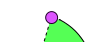
\includegraphics[scale=0.4]{rotation.png}
\end{multicols}

\renewcommand{\arraystretch}{1.5}
\begin{tabular}{|l|l|} \hline
Angular Position&$\theta_z(t)$\\ \hline
Angular Velocity&$\omega_z(t)=\frac{d\theta(t)}{dt}=\dot{\theta}$\\ \hline
Angular Acceleration&$\alpha_z(t)=\frac{d\omega(t)}{dt}=\frac{d^2\theta(t)}{dt^2}=\ddot{\theta}$ \\ \hline
\end{tabular}

}

\section{Equations of Rotation}

\frame{
\frametitle{Equations of Rotation}

You used these important relationships in your dynamics course. \vspcc

\scalebox{1}{$\vec{v}=\vec{r}\times\vec{\omega}$} 

With the planar motion assumption this vector equation can be reduced to scalar equation. \vspc

\scalebox{1}{$v=r\omega$}

}

%Section 3:
\section{Degrees of Freedom}

\frame{
\frametitle{Degrees of Freedom}

The Degrees of Freedom is the number of independent motions that exist in a system. \vspc

OR \vspc

The Degrees of Freedom is the minimum number of coordinates required to completely describe motion or state of the system.


}

%Section 4:
\section{DOF Examples}

\frame{
\frametitle{DOF Examples}

Find the degrees of freedom for each of the following systems. \vspcc

\scalebox{.7}{Wittener Metronome \hspace{10mm}Passenger Aircraft \hspace{10mm} Ackermann Steeting Mechanism} \vspc
\includegraphics[scale=.25]{Wittner_metronome.jpg} \hspc \includegraphics[scale=.125]{airbus_a320.jpg} \hspc 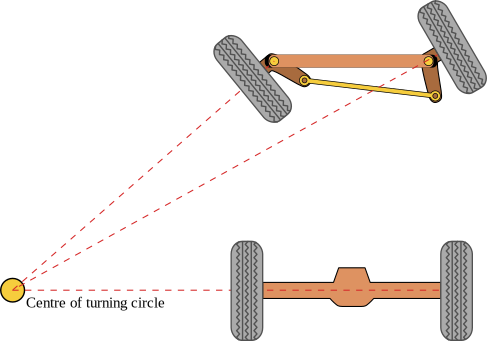
\includegraphics[scale=.25]{Ackermann_turning.png}

{\tiny \href{https://en.wikipedia.org/wiki/Metronome}{Image: Wikipedia}  \hspace{20mm}\href{https://en.wikipedia.org/wiki/Airliner}{Image: Wikipedia} \hspace{20mm}\href{https://en.wikipedia.org/wiki/Ackermann_steering_geometry}{Image: Wikipedia} }
}	
	
\end{document}



